% !TEX encoding = UTF-8 Unicode

%------------------------------------
%	PACKAGES AND OTHER DOCUMENT CONFIGURATIONS
%------------------------------------
\documentclass[letterpaper,11pt]{article}
\usepackage[utf8]{inputenc}
\usepackage[T1]{fontenc}
\usepackage{textcomp}
\usepackage{lmodern}
\usepackage[spanish,mexico]{babel} 
\usepackage{graphicx}
\usepackage{subcaption}
\usepackage{float}
\usepackage{blindtext}
\usepackage{fullpage}
\usepackage{amssymb}
\usepackage{mathtools}
\usepackage{algorithm}
\usepackage[noend]{algpseudocode}
\usepackage{nccmath}
\usepackage{enumerate}
\usepackage[none]{hyphenat}
\usepackage{amsmath}
\usepackage{graphicx}
\usepackage{wrapfig}
\usepackage[colorinlistoftodos]{todonotes}
\usepackage[normalem]{ulem}
\useunder{\uline}{\ul}{}
\setlength{\parskip}{2mm}

\begin{document}

\begin{titlepage}

\newcommand{\HRule}{\rule{\linewidth}{0.5mm}} % Defines a new command for the horizontal lines, change thickness here

\center % Center everything on the page
 
%----------------------------------------------------------------------------------------
%	HEADING SECTIONS
%----------------------------------------------------------------------------------------

\textsc{\Large Universidad de Chile, Departamento de Ingeniería Eléctrica}\\[1.5cm] % Name of your university/college
\textsc{\Large Señales y Sistemas I}\\[0.5cm] % Major heading such as course name
\textsc{\large EL-3005-2}\\[0.8cm]
\textsc{\Large Proyecto 1}\\[0.5cm] % Minor heading such as course title

%----------------------------------------------------------------------------------------
%	TITLE SECTION
%----------------------------------------------------------------------------------------

\HRule \\[0.4cm]
{ \huge \bfseries Estudio de Técnicas de Procesamiento de Señales en Sistemas de Sonar}\\[0.1cm] % Title of your document
\HRule \\[1.5cm]
 
%----------------------------------------------------------------------------------------
%	AUTHOR SECTION
%----------------------------------------------------------------------------------------

\begin{minipage}{0.4\textwidth}
\begin{flushleft} \large
\emph{Autor:}\\
Felipe \textsc{Lucero}\\
19.528.232-3 % Your name
\end{flushleft}
\end{minipage}
~
\begin{minipage}{0.4\textwidth}
\begin{flushright} \large
\emph{Profesor:} \\
Jorge F. Silva
\\
[1.0cm]
\emph{Auxiliar:}\\
Roberto Rojas\\
\end{flushright}
\end{minipage}\\[2cm]

% If you don't want a supervisor, uncomment the two lines below and remove the section above
%\Large \emph{Author:}\\
%John \textsc{Smith}\\[3cm] % Your name

%----------------------------------------------------------------------------------------
%	DATE SECTION
%----------------------------------------------------------------------------------------

{\large \today}\\[2cm] 


\vfill 

\end{titlepage}

\newpage
\tableofcontents

\newpage

\section{Descripcion del Problema}

SONAR (\textit{\textbf{S}ound \textbf{N}avigation \textbf{A}nd \text{R}anging}) es una técnica de detección de objetos mediante el uso de ondas sonoras. El principio básico del SONAR se basa en la transmisión de una determinada señal acústica, y su posterior recepción debido a la reflexión de dicha onda con algún objeto en el ambiente. Formalente, considere $x_{a}(t)$ con $t$ $\in$ $\Re$, la señal transmitida e $y_{a}(t)$ la señal recibida dada por el siguiente modelo:

\begin{equation}
y_{a}(t) = \alpha(d)x_{a}(t-t_{d}) + w_{a}(t)
\label{modelo}
\end{equation}

Donde $|\alpha(d)| <  1$  denota la pérdida de energía de la señal emitida, $w_{a}(t)$ un ruido aditivo, $d$ la distancia al objeto y $t_{d}$ el tiempo que tomo la señal en ir y volver al emisor/receptor. Posteriormente, $x_{a}(t)$ e $y_{a}(t)$ son muestradas a una tasa $T_{s} = \frac{1}{F_{s}}$ acorde al toerema del muestreo, con el fin de procesar ambas señales y determinar el retardo temporal en la señal recibida. En consecuencia, las señales resultantes a tiempo discreto entán dadas por:


\begin{equation}
x(n) = x_{a}(nT_{s})
\end{equation}

\begin{equation}
y(n) = y_{a}(nT_{s}) = \alpha(d)x_{a}(nT_{s}-DT_{s}) + w_{a}(nT_{s})
\label{modelo2}
\end{equation}

\begin{equation}
= \alpha(d)x(n-D) + w(n)
\label{modelo3}
\end{equation}

donde $t_{d} \approx DT_{s}$. Finalmente, el problema consiste en determinar el retardo $D$ a partir de las señales $x(n)$ e $y(n)$.

\section{Desarrollo}

A continuación se describen una serie de análisis a realizarse con el objetivo de entender el procesamiento de las señales del SONAR.

\subsection{Relación con la correlación cruzada}

Como se planteó en las ecuaciones \eqref{modelo}, \eqref{modelo2} y \eqref{modelo3}, es de esperarse que la señal recibida $y_{n}$ sea muy parecida a $x(n)$, solo desplazada en D. Es decir, al realizar la correlación cruzada de las señales, se esperará un máximo en $r_{xy}(l)$ con $l$ muy relacionado con $D$.\par

Un ejemplo de esto se puede ver en las siguientes figuras:


\begin{figure}[H]
\centering
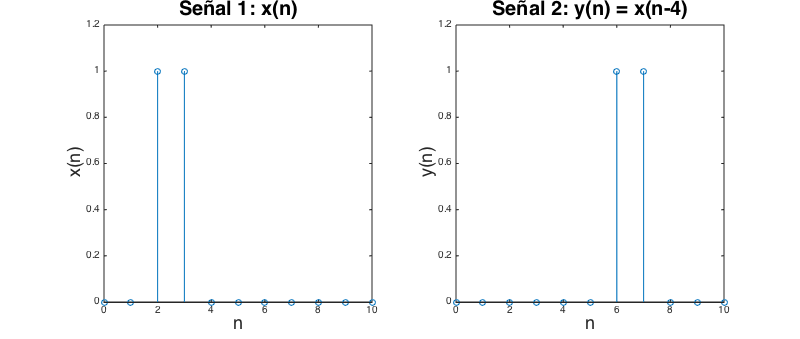
\includegraphics[width=1.0\textwidth]{img/parte_a/senales.png}
\caption{Dos señales, donde $y(n)$ es $x(n)$ desplazada en $k = 4$}
\label{desplazamiento}
\end{figure}

\begin{figure}[H]
\centering
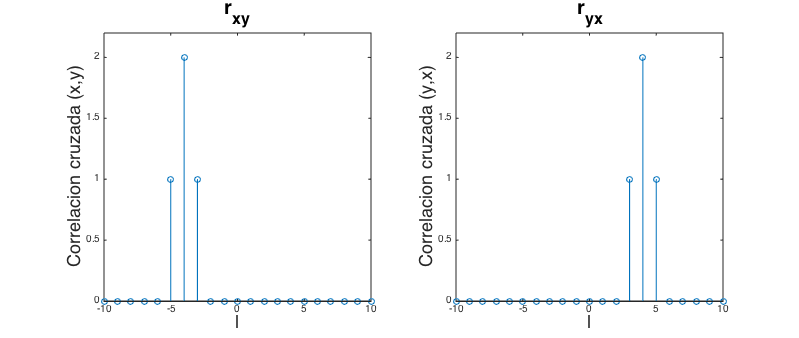
\includegraphics[width=1.0\textwidth]{img/parte_a/correlaciones.png}
\caption{Correlación cruzada entre las señales de la figura \ref{desplazamiento}, se aprecia el máximo en $l = \pm4$}
\label{correlacion}
\end{figure}

En la figura \ref{correlacion} se aprecia que el máximo se encuentra en $l = \pm 4$, que es justamente el desplazamiento relativo entre $x(n)$ y $y(n)$.

Con este análisis se corroborar que la técnica de la correlación cruzada es una buena técnica para encontrar el desplazamiento de la señal $D$.\par

Conociendo $D$, y utilizando la relación:

\begin{equation}
t_{d}\approx DT_{s}
\end{equation}

se podrá conocer el tiempo de retardo. Sabiendo que la velocidad de propagación del sonido en el mar es $ v = 1513 m/s$, se tendrá que:

\begin{equation}
d = \frac{vt_{d}}{2} \approx \frac{vDT_{s}}{2}
\end{equation}

Con esto explicado, se puede obtener la distancia al objeto

\subsection{Análisis a un set de datos conocidos}

Sabiendo el método para determinar la distancia, se puede aplicar esta técnica a datos conocidos. \par

Se considera una situación donde se emiten señales sonoras en todas direcciones ($360^{\circ}$), luego se reciben las señales, con ruido y perdida de energía.

La señal emitida es de tipo Gaussiana de la forma:

\begin{equation}
x_{a}(t) = \sqrt{\frac{20}{\sqrt{\pi}\sigma F_{s}}} exp\Bigg( -\frac{1}{2\sigma^2}(t-\mu)^2 \Bigg)
\end{equation}

donde $F_{s} = kHz$,$\mu = 0.6s$ y $\sigma = 0.1s$

Se proporcionan 7 sets de datos $(Y_{k},Phi_{k})_{k=1...7}$, cada uno asociado a un entorno o escenario particular. Cada matriz $Y_{k}$ corresponde a la señal (de largo $N =10000$) para cada angulo (alrededor de 320, dependiendo del set de datos).\par

Con esto, se determina el entorno de la forma:

\begin{algorithm}[H]
\begin{algorithmic}
	\State $k \gets i \in (1..7)$
    \State Inicializar $x(n)$ como lista, funcion gaussiana
    
	\For{$Phi_{k}(i)$}
		\State $r_{i}$ = correlacion cruzada entre $Y_{l}(i,:)$ y $x(n)$
		\State $D_{i}$ = indice del máximo de r	
    \EndFor
    
    \State $distancia_{i}$ = velocidad$\cdot T_{s} \cdot D_{i}$ / 2
\end{algorithmic}
\end{algorithm}




Así se obtienene un arreglo de distancias para cada ángulo. obteniendo un par coordenado ($\phi_{k}$,$\rho_{k}$). Los resultados de este desarrollo, se encuentran en la siguiente sección.

\subsection{Respuesta segun la ganancia otorgada}

Naturalmente, se espera algun ruido adicional y una pérdida adicional de anergía a la hora de recibir la señal, como se aprecia en la ecuacion \eqref{modelo}, es por esto que es necesario algún tipo de amplificación, así la energía de la señal es superior y será más facil reconocerla. Si el ruido ambiente es mayor, entonces es necesario una mayor amplificación para obtener resultados útiles.\par

En este caso, la señal emitida será de la forma:

\begin{equation}
x_{G} = G\cdot x(n)
\end{equation}

Para simular la señal recibida, se utilizará la función preimplementada \texttt{data\_gen.m}, que simula parámetros como.

\begin{itemize}

\item $k$ : Ambiente a utilizar

\item $\sigma^2$ : Ancho de la señal emitida (varianza)

\item $\sigma_{w}^2$ : Varianza del ruido ambiente

\item $G$ : Ganancia de la señal

\end{itemize}

Para este informe, se utilizará $\sigma^2 = 0.01$ y $\sigma_{w}^2 = 50$ y se evaluará el desempeño de la técnica, según el valor de la ganancia $G$, para esto se utilizará el indicador ruido-señal:

\begin{equation}
\epsilon_{G,k} = \frac{||\hat{d}_{\phi,k} - d_{\phi,G,k}||_{2}}{||\hat{d}_{\phi,k}||_{2}}
\end{equation}

donde $d_{\phi,G,k}$ es un vector que posse la distancia detectada para cada angulo, en el escenario k, utilizando una señal transmitida con ganancia $G$, $\hat{d}_{\phi,k}$ son las distancias reales del escenario (conocidas) y $||x(n)||_{2} = \sqrt{\sum_{k} |x(k)|^{2}}$. Se generarán curvas $\epsilon_{G,k}$ vs $G$, para cada uno de los 7 escenarios posibles, con $G \in (0.5...90)$. Los resultados de este análisis se encuentran en la sección de resultados.


\subsection{Respuesta de la señal segun el ancho de la señal emitida}

En esta parte se estudiará el comportamiento o respuesta de la señal según el ancho de la señal $x(n)$ emitida.\par

En teoría, la respuesta de la señal debería depender de la frecuencia de la señal de incidencia, por una posible relación de dispersión en el mar y la forma de los objetos a detectar. Los componentes armónicos de la señal emitida (Gaussiana), dependen directamene de la varianza (ancho) de esta, por la Transformada de Fourier de una gaussiana (mientras más angosta, más componentes en frecuencia se necesitan), como se aprecia en la siguiente figura.


\begin{figure}[H]
\centering
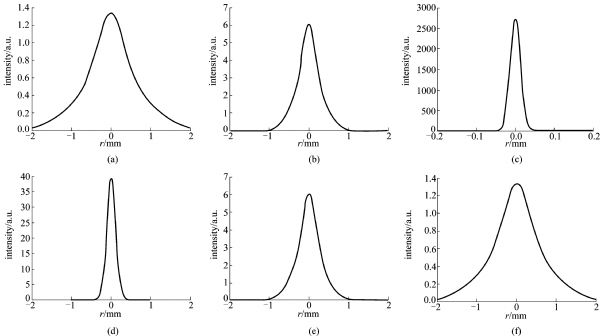
\includegraphics[width=1.0\textwidth]{img/parte_d/fourier.jpg}
\caption{Arriba: Señales continuas gaussianas con diferentes anchos. Abajo: Transformadas de fourier para las gaussianas de arriba}
\label{correlacion}
\end{figure}

\section{Resultados}



\section{Análisis}

\section{Conclusiones}




%\begin{wrapfigure}{r}{0.5\textwidth}
%\vspace{-50pt}
%\begin{center}
%\includegraphics[width=0.5\textwidth]{img/interpol1.png}
%\includegraphics[width=0.5\textwidth]{img/interpol2.png}
%\end{center}
%\vspace{-20pt}
%\caption{Interpolación de una función Lorentziana. Arriba: 5 puntos equiespaciados. Abajo: 12 puntos elegidos al azar}
%\vspace{-100pt}
%\label{interpol1}
%\end{wrapfigure}





%\newpage
%\begin{figure}[H]
%\centering
%\includegraphics[width=1.1\textwidth]{img/lagrange1.png}
%\caption{Interpolación del polinomio de Lagrange para varios puntos equiespaciados}
%\label{dif1}
%\end{figure}
%
%\begin{figure}[H]
%\centering
%\includegraphics[width=1.1\textwidth, height=6.5cm]{img/spline1.png}
%\caption{Interpolación Spline para varios puntos equiespaciados}
%\label{dif2}
%\end{figure}





\end{document}